\chapter{Previous Works}\label{chapter:prev_works}
\newcommand{\cprob}[2]{P(#1 | #2)}
The area of computational morphology is wide and rich with publications. Approaches to computational morphology can be roughly classified into 3 basic categories:
\begin{enumerate}
\item Unsupervised morphology learners: algorithms which use solely plain-text corpora or word-lists as their input.

\item Supervised systems and hand-built systems. They require annotated corpora or manually created rules together with large vocabularies.

\item Semi-supervised and resource-light approaches. The individual approaches vary in the amount and form of human supervision. The forms of human supervision may include providing data such as inflected word forms, paradigms, affix lists, phonological rules etc. Human supervisor may also be employed in an iterative training process by being asked to interact in each iteration of the learning process.
\end{enumerate}

In this chapter, some of the existing systems are described, with main focus on the unsupervised and semi-supervised methods.

\section{Creating analysers by experts}
The two most commonly used approaches to creating hand-made morphology analysers are 2-level morphology \citep{Koskenniemi83, Karttunen03} and the so-called ``engineering approach''.

\subsection{Two-level morphology (2LM)}
2LM is a popular formalism, which works with two levels of representation of words: an abstract \emph{lexical level} and a concrete \emph{surface level}, for example:
\begin{quote}\begin{flushleft}
\tt 
b a b y + 0 s\\
b a b i 0 e s
\end{flushleft}
\end{quote} with an inline notation 
\begin{quote}\begin{flushleft}
\tt 
b:b a:a b:b y:i +:0 0:e s:s
\end{flushleft}
\end{quote}
relates the lexical (upper) and surface (lower) form of the word \e{babies} . The + character denotes the morpheme boundary, 0 is an empty string (there has to be a 1:1 correspondence between characters on each level). The two levels are related by declarative context-sensitive rules such as: 
\begin{quote}\begin{flushleft}
\tt 
y:i <= \_ +:0 s:s\\
0:e <= y:i +:0 \_ s:s
\end{flushleft}
\end{quote}
The rules above describe changing of \e{y} to \e{i} before the morpheme boundary followed by \e{s} and insertion of \e{e} between \e{i} and \e{s} (in the specified context). The underscore sign denotes the position where the change is taking place.

The designer of the analyser specifies the rules and a network of lexicons containing morphemes in their lexical form. The network also specifies basic morphotactics of morphemes in the lexicons. Rules and lexicons are then compiled into a finite-state transducer. The formalism is powerful enough to express  most of the phonological and morphological processes, although their description by the rules is not always straightforward.

\subsection{Engineering approach}\label{sec:engineer}
The engineering approach, represented by \citep{hajic-2004-hab}, models morphology as a purely concatenative process. Changing parts of the stem are moved to the suffixes and as a result, high number of paradigms emerge. For example, to model the English past tense one would need to create paradims as (\e{0, ed}), (\e{0, ped}), (\e{0, ted}), (\e{y, ied}) etc.
 Table \ref{table:matka_eng} shows how would an ``engineering'' paradigm for the word \gloss{matka}{mother} look like. (For comparison with the ``linguistic'' paradigm, see Table \ref{table:matka}). 
 
 Positive attributes of the approach are easy implementation, high speed and a well readable morphology specification.

\begin{table}[htb]
\begin{center}
\begin{tabular}{lll}
\toprule \bf Case & \bf Singular & \bf Plural \\ \midrule
nom & mat + ka &  mat + ky \\
gen & mat + ky &  mat + ek \\
dat & mat + ce &  mat + kám\\
acc & mat + ku &  mat + ky \\
voc & mat + ko &  mat + ky \\
loc & mat + ce &  mat + kách \\
inst & mat + kou & mat + kami \\
\bottomrule
\end{tabular}
\end{center}
\caption{\label{table:matka_eng} Engineering approach paradigm for \gloss{matka}{mother}.}
\end{table}

\section{Unsupervised algorithms}
This section presents two representatives of the unsupervised approaches: Goldsmith's Linguistica \citep{goldsmith01}, which returns partial paradigms called \emph{signatures} and Morfessor \citep{creutz-lagus-2002, creutz-lagus-2005, creutz07}, which induces morphemic segmentation of plain-text corpora. Paramor \citep{monson09}, the unsupervised algorithm I have extended in this thesis, is described separately in Chapter \ref{chapter:paramor}.

\subsection{Linguistica}
\cite{goldsmith01} presents Linguistica, an unsupervised approach based on minimum description length (MDL). Basic idea of the approach is to find a morphology model which is compact and allows compact representation of the corpus. More precisely, a model that minimises the sum of the compressed size of the corpus and the compressed size of the model. Assumption is that the model will be close to reality due to the economy of languages. 

Morphology model consists of a stem list, suffix lists and a set of \emph{signatures}. A signature contains stems and suffixes (more precisely, pointers to the respective lists). Their presence together means that all combinations of stems and suffixes in the signature are possible in the given language. A stem can be present only in one signature, occurrence of a suffix in more signatures is possible. A sample of several signatures (without stems) can be found in Table \ref{table:goldsmith-signatures}.

To be able to analyse a word as a stem and more than one suffix, Goldsmith introduces \emph{complex stems}, which consist of three pointers: to a signature, a stem and a suffix. For example, the word \emph{workings} would be analysed as a complex stem \emph{working} (pointers to: stem \emph{work}, suffix \emph{ing}, signature for \emph{working}) + suffix \emph{s}. The algorithm works roughly as follows:
\begin{enumerate}
\item Words are divided into stems and suffixes using probability based heuristics. Signatures are created according to these splits. One of the heuristics is the following: Consider all the tails up to the length 6 and score them by the measure:
\[\frac{C(n_1n_2 \dots n_k)}{N_k} ~ \log \frac{C(n_1n_2 \dots n_k)}{C(n_1) C(n_2) \dots C(n_k)}\]
where $n_1,n_2 \dots n_k$ are individual characters of the tail, $N_k$ denotes the number of all tails of length $k$ and $C(x)$ denotes count of $x$. Top 100 tails ranked by this measure are selected as the candidate suffixes.
\item Signatures containing only one stem or only one suffix are discarded. 
\item Two types of modifications to the initial morphology are tested and applied if they decrease the description length:
\begin{itemize}
\item Splitting a suffix into two if the suffix is a concatenation of two already known suffixes. For example, the suffix \e{ings} is split into \e{ing} and \e{s}.
\item If all the suffixes of the signature begin with the same letter, the letter can be moved from the suffixes to the stems. For example, \e{te.ting.tes} may become \e{e.ing.es}.
\end{itemize} 
\end{enumerate} 

An example of Linguistica's output is shown in Table \ref{table:goldsmith-signatures}. Limitation of Linguistica is that it does not capture stem-internal changes and point-of-affixation phonological/graphemic changes. It also disregards the context of the words, which may be a useful source of information, as shown by the work of \cite{yarowsky00}, described in Section \ref{y_and_w}.

\begin{table}[h]
\begin{center}
\begin{tabular}{rlrrlr}\toprule
\bf Rank     & \bf Signature & \bf  \#Stems & \bf Rank & \bf Signature & \bf \#Stems \\\midrule
1	 & 	NULL.ed.ing		& 	69	 & 16	 & 	e.es.ing	 & 	7	 \\
2	 & 	e.ed.ing		& 	35	 & 17	 & 	NULL.ly.ness	 & 	7	 \\
3	 & 	NULL.s	 		& 	253	 & 18	 & 	NULL.ness	 & 	20	 \\
4	 & 	NULL.ed.s		& 	30	 & 19	 & 	e.ing	 & 	18	 \\
5	 &  NULL.ed.ing.s	& 	14	 & 20	 & 	NULL.ly.s	 & 	6	  \\
6	 & 	's.NULL.s	 	& 	23	 & 21	 & 	NULL.y	 & 	17	 \\
7	 & 	NULL.ly	 		& 	105	 & 22	 & 	NULL.er	 & 	16	 \\
8	 & 	NULL.ing.s		& 	18	 & 23	 & 	e.ed.es.ing	 & 	4\\
9	 & 	NULL.ed			& 	89	 & 24	 & 	NULL.ed.er.ing	 & 	4\\
10	 & 	NULL.ing		& 	77	 & 25	 & 	NULL.es	 & 	16\\
11	 & 	ed.ing			& 	74	 & 26	 & 	NULL.ful	 & 	13\\
12	 & 	's.NULL			& 	65	 & 27	 & 	NULL.e	 & 	13\\
13	 & 	e.ed			& 	44	 & 28	 & 	ed.s	 & 	13\\
14	 & 	e.es			& 	42	 & 29	 & 	e.ed.es	 & 	5\\
15	 & 	NULL.er.est.ly	& 	5	 & 30	 & 	ed.es.ing	 & 	5\\\bottomrule
\end{tabular}
\end{center}
\caption{\label{table:goldsmith-signatures} Top English signatures produced by Linguistica}
\end{table}

\subsection{Morfessor}
Morfessor is a family of algorithms for unsupervised morpheme segmentation developed by Mathias Creutz and Krista Lagus. Their work progressed from the relatively simple Morfessor-baseline \citep{creutz-lagus-2002} to the latest Morfessor-MAP \citep{creutz07} with a relatively complex probabilistic model. Unlike Linguistica, Morfessor is capable of dividing words into an unlimited number of morphs. This is motivated by agglutinative languages such as Finnish, where words composed of high number of morphemes are frequent. In this section, most of the attention will be focused on Morfessor-MAP, as the other models can be viewed as its simplifications. Short description of the baseline algorithm will be presented as well to demonstrate the basic idea.

Morfessor-baseline uses MDL to evaluate its analyses. It starts with each word as a separate morph. Then for each word, all possible splits into two parts are examined. If one of the parts is an already existing morph and the split decreases the compressed corpus size, the split is accepted and the splitting attempts continue recursively. When the whole corpus is analysed in this way, randomly selected words are merged and resplit.

Such an approach doesn't take into account the morph's function as a prefix, stem or suffix. Therefore, after seeing \emph{write} in the corpus and analysing \emph{writes} as \emph{write} + \emph{s}, \emph{s} is recognised as a morph which enables the analysis of \emph{storm} as \emph{s} + \emph{torm}. To address this issue, later versions of Morfessor use HMM to assign function tags to morphs. There are four such tags: \emph{prefix} (PRE), \emph{stem} (STM), \emph{suffix} (SUF) and \emph{nonmorpheme} (NON). The nonmorpheme category helps to tackle a common problem of MDL-based approaches -- marking frequent syllables or a word fragments as morphemes. Successful identification of such strings allows to keep them internally for the sake of economical representation of the corpus and at the same time dealing with them when constructing the final analysis. Morfessor-MAP's analysis of a word is a hierarchical structure, such as [[straight[for ward]][ness]]. When creating the final analysis, the structure is expanded to the finest resolution not containing nonmorphemes. So, if \emph{for} is tagged as NON, the [[straight forward][ness]] analysis is presented as a result.

Morfessor-MAP uses a generative probabilistic model and Bayesian \emph{maximum a posteriori} (from here comes the MAP acronym) approach to evaluate quality of the analyses and search for the best one. The approach can be described shortly by the following formula:
\[
\argmax_{\mathbb{M}} P(\mathbb{M} | \mathit{corpus}) = \argmax_{\mathbb{M}} P(\mathit{corpus} | \mathbb{M}) \cdot P(\mathbb{M})
\]
$\mathbb{M}$ stands for a model of the language, which expresses properties of grammar and lexicon. In order to use the formula, a prior probability distribution has to be defined for the model, as well as the posterior $P(\mathit{corpus} | \mathbb{M})$. The posterior is defined by the Hidden Markov Model (HMM):
\[
P(\mathit{corpus} | \mathbb{M}) = \prod_{j=1}^{W} \left[ \cprob{{C_j}_1}{{C_j}_0} \prod_{k=1}^{n_j} \cprob{\mu_{jk}}{C_{jk}} \cprob{C_{j(k+1)}}{C_{jk}}\right] 
\]

where $W$ denotes the token count of the corpus, $\mu_{jk}$ the $k$-th morph in the $j$-th token and $C_{jk}$ its tag.

The prior $P(\mathbb{M})$ takes into account various features of morphs: their (hierarchical) structure, frequency, length, left and right perplexity. The perplexities express unpredictability of the morph's left/right context. The assumption is that prefixes can be attached to a big number of stems and therefore their right perplexity is high and analogically for suffixes and the left perplexity. This assumption leads to the definition of class probabilities $\cprob{C_{jk}}{\mu_{jk}}$ for PRE and SUF based on right/left perplexity. Details about the generative model can be found in \cite[pp. 9--16]{creutz07}.

The search for the most probable hypothesis is heuristic and uses the Morfessor-baseli\-ne as the initial hypothesis. It can be summarised as follows:
\begin{enumerate}
\item Initialisation of segmentation by Morfessor-baseline
\item Splitting of morphs
\item Joining of morphs using a bottom-up strategy
\item Splitting of morphs
\item Resegmentation of the corpus using Viterbi algorithm and reestimation of probabilities until convergence
\item Repetition of steps 3–5 once
\item Expansion of the morph substructures to the finest resolution that does not contain non-morphemes
\end{enumerate}
See \cite{creutz-lagus-2005} for detailed description of the search procedure.

Evaluation on the morpheme segmentation task using gold standard showed that Morfessor outperforms Goldsmith's Linguistica on both English and Finnish data. As one may expect, on the Finnish corpus the performance gap was wider.

\subsection{Semi-supervised learning based on Morfessor}\label{section:semisup_morfessor}

\cite{kohonen-etal-2010} improve Morfessor's performance using correctly segmented words (1000+ for English, 100+ for Finnish) as a seed. The seeded algorithm achieved significant improvement in recall for both languages, accompanied by only a slight drop in precision.

\cite{tepper10} use hand-written transformation rules to capture allomorphy and improve Morfessor's segmentation. Output of the Morfessor-MAP algorithm is used as the initial corpus segmentation. The splits are then re-estimated using an HMM with underlying forms of the morphs as a hidden variable. An underlying form is a single representation of a set of allomorphs. The system was tested on English and Turkish and outperformed the Morfessor-MAP baseline on both languages.

\section{Combination of multiple sources of information}
Works by \cite{yarowsky00} and \cite{schone01} aim at using more sources of information such as string similarity and context similarity to create a combined classifier which achieves significantly higher quality than its individual parts. The approach of \cite{yarowsky00} is described in the following section as a representative of this class of approaches.

\subsection[Yarowsky and Wicentowski (2000)]{\cite{yarowsky00}}\label{y_and_w}
\cite{yarowsky00} present an algorithm for aligning inflections to lemmas. They evaluate the algorithm on past tense of verbs and show that it is capable of handling irregular forms. The system works iteratively and ranks potential lemmas and morphological tags for each word by 4 different measures:
\begin{enumerate}
\item Frequency similarity. This measure computes the word's relative frequencies with respect to its hypothetical inflections given the candidate tag and lemma. The candidate tag scores well if the frequencies fit the expected distributions of tag-to-tag ratios. For example, \e{singed} as a candidate for past tense of \e{sing} will receive a low score, as the frequency ratio \e{singed}/\e{sing} is 0.007, while the overall ratio of \e{VBD}/\e{VB} is 0.85. (The ratio \e{sang}/\e{sing} is 1.19.) The estimators of the tag-to-tag ratios can be trained on the regular forms only, as according to the authors' observations, the ratios of the irregular forms follow similar distributions.

\item Context similarity measure assumes that different forms of the same lemma occur in similar context. The context is extracted using ``a set of simple regular expressions over small closed-class parts of speech'' with an aim to find subjects and objects of the verbs. The context words are lemmatised using the output from the previous iterations, which helps to reduce sparsity.

\item Weighted Levenshtein distance \citep{levenshtein66}, capable of setting different costs for individual characters or character classes. It uses a cost matrix which in the first iteration is set to less penalise changing vowels to other vowels. Alternatively, a `trained' matrix from a related language can be used as the initial setting. In the following iterations, the matrix is re-estimated from the $<$inflection, lemma$>$ alignments from the previous iteration. 

\item Probabilistic function mapping inflections to lemmas, modelling stem-final pho\-nological changes. The probabilistic model, called MorphTrans, is trained on the output of the previous iteration. In the first iteration, the probabilities depend on the modified Levenshtein distance.
\end{enumerate}

\noindent The algorithm requires a number of resources:
\begin{enumerate}
\item Large unannotated corpus.
\item List of the language's parts of speech together with their canonical suffixes. 
\item List of open class base forms. It is typically obtainable from dictionaries.
\item A rough mechanism for identifying the candidate parts of speech
of the remaining vocabulary, not based on morphological analysis.
\item List of consonants and vowels for given language.
\end{enumerate}

\noindent Classifier combination techniques are used to merge the results of the four measures. As the iterations proceed, the MorphTrans component gains relative weight as it becomes better trained. The system achieved excellent results on correctly identifying lemmas of English past tense verbs. Its accuracy on regular verbs was almost 100\%, while achieving 80\% accuracy on the irregular ones.

The approach has shown that classifiers which are working with various sources of information and not accurate individually can be successfully combined into a high-accuracy system. Table \ref{table:yarowsky_table} shows the scores of the candidate lemmas for the word \e{shook} in the first iteration (except for the last column, which shows the score by the converged MorphTrans model). Although the correct lemma \e{shake} was ranked first only by one of the four basic measures, it was successfully identified by the overall consensus similarity measure.

\begin{table}[h]
\centering
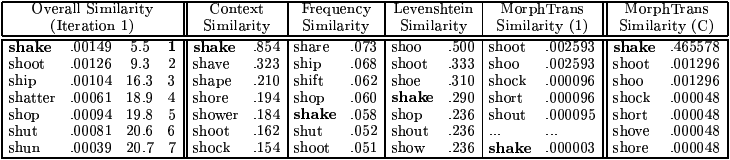
\includegraphics[scale=0.75]{yAw_table.png}
\caption{Candidate lemmas of the word \e{shook}. Source: \citep{yarowsky00}}
\label{table:yarowsky_table}
\end{table}

However, with highly inflected languages and other parts-of-speech than verbs, using this approach may be problematic. First, the context similarity measure assumes that inflections of the same lemma occur in similar context. Which works well with English verbs, as they have the same subcategorisation requirements in the past and in the present tense. On the other hand, if we consider Czech nouns, their accompanying adjectives exhibit agreement in case and number and therefore will be in a different form for differently inflected nouns (e.g. \e{zelená tráva} `green grass' (sg. nom.) vs. \e{zelenou trávou} (sg. ins.)).

Second, providing a list of all parts-of-speech and their canonical suffixes for languages with rich inflection would be more labour intensive as there can be hundreds or thousands of tags in the given language and less helpful, as there is great suffix homonymy in such languages. For example, \cite{feldman-hana-2010-rodopi} illustrate the homonymy of Czech using the suffix \e{a}, which has ``about 19 different meanings.'' (See Table \ref{table:ambiguity-a}) 

\begin{table}[h]
\begin{center}
\begin{tabular}{llll}

%
\toprule
\bf Form      & \bf Lemma    & \bf Gloss  & \bf Category                \\ 
\midrule
m\v{e}st-a    & m\v{e}sto    & town      & noun neuter sg gen           \\
          &          &                   & noun neuter pl nom (voc)     \\
          &          &                   & noun neuter pl acc           \\
t\'{e}m-a     & t\'{e}ma     & theme     & noun neuter sg nom (voc)     \\
          &          &                   & noun neuter sg acc           \\
\v{z}en-a     & \v{z}ena     & woman     & noun feminine sg nom            \\
p\'{a}n-a     & p\'{a}n      & man       & noun masculine anim sg gen      \\
          &          &                   & noun masculine anim sg acc      \\
ostrov-a  & ostrov   & island            & noun masculine inanim sg gen    \\
p\v{r}edsed-a & p\v{r}edseda & president & noun masculine anim sg nom      \\
vid\v{e}-l-a  & vid\v{e}t    & see       & verb past feminine sg           \\
          &          &                   & verb past neuter pl          \\
vid\v{e}-n-a  &          &               & verb passive feminine sg        \\
          &          &                   & verb passive neuter pl       \\
vid-a     &          &                   & verb transgressive masculine sg \\
dv-a      & dv-a     & two               & numeral masculine sg nom        \\
          &          &                   & numeral masculine sg acc        \\
\bottomrule
\end{tabular}
\end{center}
\caption{\label{table:ambiguity-a}Homonymy of the \e{a} ending in Czech (from \cite{feldman-hana-2010-rodopi})}
\end{table}

\subsection{Extended MorphTrans model as a supervised learner}
\cite{wicentowski04} extends the probabilistic model developed in \citep{yarowsky00} to handle prefixation and stem-internal vowel change. The extended model is called the WordFrame (WF) and it is used for supervised learning with training data in the form of \emph{$<$inflection, lemma$>$} pair list. Optional resources are a prefix list and a suffix list. Inflection is modelled as 5 possible transformations of the lemma: 
\begin{enumerate}
\item Adding a prefix $\psi_p'$ from the prefix list.
\item Point-of-prefixation stem change $\delta_p' \rightarrow \delta_p$
\item Stem internal vowel change $\delta_v' \rightarrow \delta_v$. $\delta_v'$ and $\delta_v$ may contain more than one vowel, but they must be both non-empty or both empty.
\item Point-of-suffixation stem change $\delta_s' \rightarrow \delta_s$
\item Removing a canonical suffix (e.g. infinitival ending for verbs) $\psi_s$ and adding a suffix $\psi_s'$ from the suffix list.
\end{enumerate}

\noindent Table \ref{table:wordframe} shows differences between the MorphTrans and the WordFrame model on the example of \e{kept} $\rightarrow$ \e{keep} transformation. The WordFrame is capable of capturing the stem internal change \e{e} $\rightarrow$ \e{ee}. Such rule is a better generalisation than the stem final change \e{p} $\rightarrow$ \e{ep}, for example it would work for \e{met} $\rightarrow$ \e{meet}.
\begin{table}[h]
\begin{center}
\begin{tabular}{llllllll}
\toprule
& $\psi_p'$    & $\delta_p' \rightarrow \delta_p$ & $\gamma_p$ & $\delta_v' \rightarrow \delta_v$ & $\gamma_s$ & $\delta_s' \rightarrow \delta_s$ & $\psi_s' \rightarrow \psi_s$     \\ 
\midrule
MorphTrans & N/A & N/A & N/A & N/A & ke & p $ \rightarrow$ ep & t $ \rightarrow \lambda$ \\
WordFrame & & & k &  e $\rightarrow$ ee & p &  & t $\rightarrow \lambda$\\
\bottomrule
\end{tabular}
\end{center}
\caption{\label{table:wordframe} Mapping \e{kept} $\rightarrow$ \e{keep} analysed by MorpTrans and WordFrame models. Source: \cite{wicentowski04}}
\end{table}

As a whole, inflection is a transformation $\delta_p \gamma_p \delta_v \gamma_s \delta_s \psi_s \rightarrow \psi_p' \delta_p' \gamma_p \delta_v' \gamma_s \delta_s' \psi_s'$ where ($\gamma_p \delta_v \gamma_s$, $\gamma_p \delta_v' \gamma_s$) is the \emph{WordFrame}, the longest common substring with at most one vowel change. Division of the training pairs into the subparts is done deterministically by:
\begin{enumerate}
\item Removing the longest matching prefix and suffix present in the affix lists from the inflection and a canonical prefix from the stem.
\item Finding the WordFrame.
\item Remaining strings on the left and right from the WF are considered $\delta_p/\delta_p'$ and $\delta_s/\delta_s'$.
\end{enumerate}

Analysis of an unseen inflection is done probabilistically by finding the lemma maximising \[P(\delta_p \gamma_p \delta_v \gamma_s \delta_s |\delta_p' \gamma_p \delta_v' \gamma_s \delta_s') = P(\delta_v' \rightarrow \delta_v, \delta_p' \rightarrow \delta_p, \delta_s' \rightarrow \delta_s|\delta_p' \gamma_p \delta_v' \gamma_s \delta_s')\] 
Point-of-suffixation change probability $P(\delta_s' \rightarrow \delta_s|\delta_p' \gamma_p \delta_v' \gamma_s \delta_s')$ is taken from a hierarchically smoothed suffix trie created in the training phase. $P(\delta_p' \rightarrow \delta_p|\delta_p' \gamma_p \delta_v' \gamma_s )$ is retrieved from an analogous prefix trie and the vowel change probability is estimated without regard on the local context (by $P(\delta_v|\delta_v')$).

The approach was tested on inflected verb forms in 32 languages, including Czech, with very good results. The size of the training data ranged from 9 lemmas and 201 inflections for Greek to 5715 lemmas and 23786 inflections for Czech.

\section{Automatic lexicon acquisition for provided pa\-ra\-digms}
The resource-light system by \cite{feldman-hana-2010-rodopi} uses manually specified pa\-ra\-digms as an input. The paradigms are specified by suffixes and point-of-affixation stem change rules. For each word in the corpus, possible paradigms are found and only the ones supported by the highest number of forms-tokens and/or form-types are retained.

\section{Semi-supervised systems using human elicitation}
\cite{oflazer01} describe a framework for creating morphological analysers of under-resourced languages. The framework makes use of direct human supervision in combination with machine learning in an iterative process. 

Input required from a human is a definition of paradigms. A paradigm is a set of words with (almost) the same inflectional behaviour. Each paradigm contains a primary example, optional secondary examples and a lexicon. An example is defined by its \emph{citation form} (the form one would look for in a dictionary) and inflected forms together with their morphological categories. The primary example must provide inflected forms for all values of relevant categories. This is not required for the secondary examples, which may be used to show irregularities for specific category combinations. A paradigm's lexicon contains citation forms of words which (presumably) belong to the paradigm.

After paradigm definition, the examples are automatically segmented in\-to stem and affixes. (Settings described in the paper allow at most one prefix and one suffix for a stem.) All string-prefixes (substrings beginning with the first letter) of a citation form (CF) are considered candidates for the stem. The candidate minimising the sum of  edit distances to all the inflected forms is chosen as a stem $s$. Then for each inflected form (IF), the projection of the stem is found (a substring with minimal edit distance to $s$). The remaining strings at the start and the end of the IF are considered prefix/suffix. The resulting segmentation is \emph{(prefix) + CF + (suffix)}. (The citation form is used instead of the stem.)

Segmented lexical forms are then aligned to the surface form as in the example (p. 71):
\begin{center}
\texttt{un + happy + est \hspace{10pt}  shop0 + ed\\
un 0 happi 0 est \hspace{10pt} shopp 0 ed}
\end{center} 
Alignment has 3 constraints : \begin{quote}
(i) a + in the segmented lexical form is always aligned with an empty string on the surface
side, notated by 0; (ii) a consonant on one side is always aligned with a consonant or 0 on the other side, and likewise for vowels; (iii) the alignment must correspond to the minimum edit distance between the original lexical and surface forms. (pp. 70 -- 71)
\end{quote}
Aligned pairs are used by a transformation based learner to learn context-based rewrite rules which transform the lexical forms into the surface forms. The rules are in form \texttt{u -> v || lc \_ rc}, where \texttt{u} is the symbol in the lexical form, \texttt{v} is the symbol in the surface form,  \texttt{lc} and  \texttt{rc} regular expressions describing left/right context of a limited length. For the previous examples, one can get rules like:
\begin{quote}
\begin{flushleft}
\texttt{y -> i || p \_ \\ 
y -> i || p \_ + e\\
y -> i || p \_ + e s \\ 
+ -> 0 || \# u n \_ h a p\\}
\end{flushleft}
\end{quote}
(p. 71), where \# denotes a word boundary, which may be used in context definition as well. The system allows assigning categories to characters and creation of more general rules by using categories in context definitions. In the presented implementation, characters are marked as consonants or vowels and for each rule, its generalised versions is generated. For example, the rule \texttt{0 -> p || p \_ + e} (p. 72) can be generalised by 3 different rules: \begin{quote}
\begin{flushleft}
\texttt{0 -> p || CONSONANT \_ + e}\\
\texttt{0 -> p || p + \_ VOWEL}\\
\texttt{0 -> p || CONSONANT \_ + VOWEL}\\
\end{flushleft}
\end{quote}
The same rule is often generated from more than one example. Number of such examples for a rule is called rule's \emph{promise}.

Rule selection is done iteratively by selecting the best rule and applying it to the list of lexical forms. Rules are sorted according to their promise, with the exception of the segmentation rules (\texttt{+ -> 0}), which are put to the bottom of the list. (The morpheme boundary is an important context for most of the rules and should not be removed prematurely.) The topmost rule, which does not cause errors (its application does not make any lexical form to be more distant from its corresponding surface form) is selected and applied to the lexical forms. The process is iterated until all the lexical forms are transformed to their corresponding surface forms.  

Using XRCE finite-state tools, the selected rules are compiled together with the lexicon to a finite-state transducer for the paradigm. The tools can be used for testing the analyser and finding where it makes mistakes. It is possible to generate all inflected forms for a citation form or all forms with one value of a category. 

When the analysers for paradigms are unioned to create the final analyser, a more elaborate method of testing is used. An error-tolerant finite-state recognizer engine is employed to find candidates for fixing -- words in a corpus which are not accepted by the analyser, but close to an accepted form. Then the human may adjust the system by adding more examples in an attempt to fix the errors and next iteration of learning is started.

